\documentclass[a4paper,12pt]{article} % добавить leqno в [] для нумерации слева
\usepackage[a4paper,top=1.3cm,bottom=2cm,left=1.5cm,right=1.5cm,marginparwidth=0.75cm]{geometry}
%%% Работа с русским языком
\usepackage{cmap}					% поиск в PDF
\usepackage[warn]{mathtext} 		% русские буквы в фомулах
\usepackage[T2A]{fontenc}			% кодировка
\usepackage[utf8]{inputenc}			% кодировка исходного текста
\usepackage[english,russian]{babel}	% локализация и переносы
\usepackage{physics}
\usepackage{multirow}

%%% Нормальное размещение таблиц (писать [H] в окружении таблицы)
\usepackage{float}
\restylefloat{table}


\usepackage{graphicx}

\usepackage{wrapfig}
\usepackage{tabularx}

\usepackage{hyperref}
\usepackage[rgb]{xcolor}
\hypersetup{
	colorlinks=true,urlcolor=blue
}
\usepackage{pgfplots}
\pgfplotsset{compat=1.9}
%%% Дополнительная работа с математикой
\usepackage{amsmath,amsfonts,amssymb,amsthm,mathtools} % AMS
\usepackage{icomma} % "Умная" запятая: $0,2$ --- число, $0, 2$ --- перечисление

%% Номера формул
%\mathtoolsset{showonlyrefs=true} % Показывать номера только у тех формул, на которые есть \eqref{} в тексте.

%% Шрифты
\usepackage{euscript}	 % Шрифт Евклид
\usepackage{mathrsfs} % Красивый матшрифт

%% Свои команды
\DeclareMathOperator{\sgn}{\mathop{sgn}}

%% Перенос знаков в формулах (по Львовскому)
\newcommand*{\hm}[1]{#1\nobreak\discretionary{}
	{\hbox{$\mathsurround=0pt #1$}}{}}

\date{\today}

\begin{document}

\begin{titlepage}
	\begin{center}
		{\large МОСКОВСКИЙ ФИЗИКО-ТЕХНИЧЕСКИЙ ИНСТИТУТ (НАЦИОНАЛЬНЫЙ ИССЛЕДОВАТЕЛЬСКИЙ УНИВЕРСИТЕТ)}
	\end{center}
	\begin{center}
		{\large Физтех-школа физики и исследований им. Ландау}
	\end{center}
	
	
	\vspace{4.5cm}
	{\huge
		\begin{center}
			{\bf Отчёт о выполнении лабораторной работы №3.5.3}\\
			Релаксационные колебания
		\end{center}
	}
	\vspace{2cm}
	\begin{flushright}
		{\LARGE Автор:\\ Сенокосов Арсений Олегович \\
			\vspace{0.2cm}
			Б02-012}
	\end{flushright}
	\vspace{8cm}
	\begin{center}
		Долгопрудный\\
		\today
	\end{center}
\end{titlepage}
%\numberwithin{equation}{section}
\section{Введение}

\textbf{Цель работы:} изучение вольт-амперной характеристики нормального тлеющего разряда; исследование релаксационного генератора на стабилитроне.


\textbf{В работе используются:} стабилитрон СГ-2 (газонаполненный диод) на монтажной панели, амперметр, вольтметр, магазин сопротивлений, магазин ёмкостей, источник питания, осциллограф (ЭО), генератор звуковой частоты (ЗГ).

\section{Теоретические сведения}

\begin{wrapfigure}{r}{5cm}
	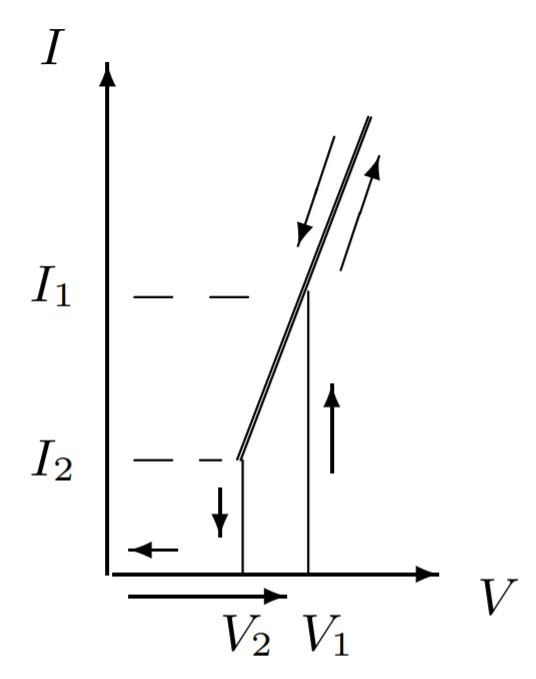
\includegraphics[width=5cm]{ris1.jpg}
	\caption{\textit{Вольт-амперная характеристика стабилитрона с последовательно включённым резистором}}
	\label{ris1}
\end{wrapfigure}

Колебательные системы, как правило, имеют два накопителя энергии, между которыми происходит её перекачка. В контуре, содержащем конденсатор и катушку индуктивности, электрическая энергия переходит в магнитную и обратно.

Встречаются, однако, колебательные системы, содержащие всего один накопитель энергии. Рассмотрим в качестве примера электрическую цепь, содержащую конденсатор и сопротивление без самоиндукции. Разряд конденсатора через сопротивление представляет собой апериодический процесс. Разряду, однако, можно придать периодический характер, возобновляя заряд конденсатора через постоянные промежутки времени. Колебания в этом случае являются совокупностью двух апериодических процессов -- процесса зарядки конденсатора и процесса его разрядки. Такие колебания называются релаксационными.

В нашей установке роль <<ключа>>, обеспечивающего попеременную зарядку и разрядку конденсатора, играет газоразрядный диод. Зависимость тока от напряжения для газоразрядной лампы не подчиняется закону Ома и характеризуется рядом особенностей (рис. \ref{ris1}). При малых напряжениях лампа практически не пропускает тока. Ток в лампе возникает только в том случае, если разность потенциалов на её электродах достигает напряжения зажигания $ V_1 $. При этом скачком устанавливается конечная сила тока $ I_1 $ -- в лампе возникает нормальный тлеющий разряд. При дальнейшем незначительном увеличении напряжения сила тока заметно возрастает по закону, близкому к линейному. Нормальный тлеющий разряд -- стабилизатор напряжения, отсюда второе название лампы -- стабиловольт.

\begin{wrapfigure}{r}{5cm}
	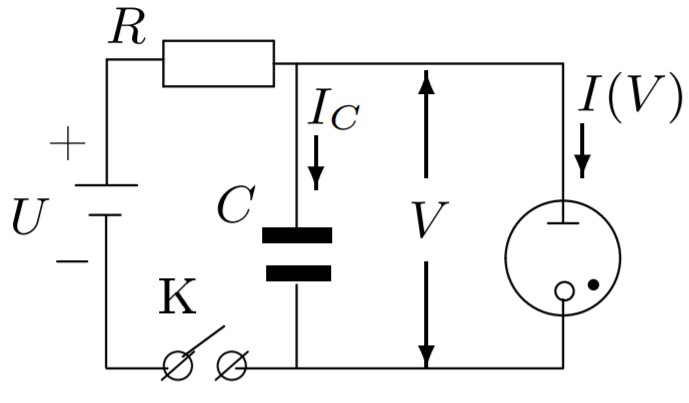
\includegraphics[width=5cm]{ris2.jpg}
	\caption{\textit{Принципиальная схема релаксационного генератора}}
	\label{ris2}
\end{wrapfigure}

Если начать уменьшать напряжение на горящей лампе, то при напряжении, равном $ V_1 $, лампа ещё не гаснет, и сила тока продолжает уменьшаться. Лампа перестанет пропускать ток лишь при напряжении гашения $ V_2 $, которое обычно существенно меньше $ V_1 $. Сила тока при этом скачком падает от значения $ I_2 $ ($ I_2 < I_1 $) до нуля.

Характеристика, изображённая на рис. \ref{ris1}, несколько идеализирована. У реальной лампы зависимость $ I(V) $ не вполне линейна.



При $ V > V_1 $ графики, соответствующие возрастанию и убыванию напряжения, не всегда совпадают. Эти отличия, впрочем, носят второстепенный характер и для нашей задачи несущественны.

Рассмотрим схему релаксационного генератора, представленную на рис. \ref{ris2}. Пусть напряжение батареи $ U $ больше напряжения зажигания $ V_1 $. В обозначениях, принятых на схеме, справедливо уравнение

\[ I_C+I(V)=\frac{U-V}{R} \]
или
\begin{equation}\label{1}
C\frac{dV}{dt}+I(V)=\frac{U-V}{R}.
\end{equation}

\begin{wrapfigure}{r}{5cm}
	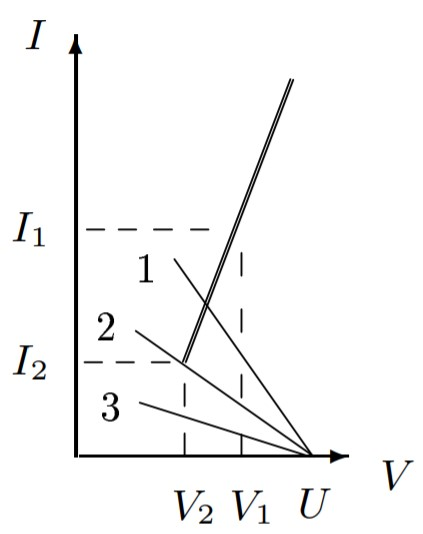
\includegraphics[width=5cm]{ris3.jpg}
	\caption{\textit{Режимы работы релаксационного генератора}}
	\label{ris3}
\end{wrapfigure}

В стационарном режиме работы, когда напряжение $ V $ на конденсаторе постоянно и $ dV/dt=0 $, ток через лампу равен

\begin{equation}\label{2}
I_\text{ст}=\frac{U-V}{R}
\end{equation}

Равенство \eqref{2} может быть представлено графически (рис. \ref{ris3}).

При разных $ R $ графики имеют вид прямых, пересекающихся в точке $ V=U, I=0 $. Область, где эти нагрузочные прямые пересекают вольт-амперную характеристику лампы, соответствует стационарному режиму -- при малых $ R $ (прямая 1) лампа горит постоянно, колебания отсутствуют. Прямая 2, проходящая через точку $ (I_2, V_2) $, соответствует критическому сопротивлению

\begin{equation}\label{3}
R_\text{кр}=\frac{U-V_2}{I_2}
\end{equation}

При сопротивлении $ R>R_\text{кр} $ нагрузочная прямая 3 не пересекает характеристику лампы, поэтому стационарный режим невозможен. В этом случае в системе устанавливаются колебания.

\begin{wrapfigure}{r}{5cm}
	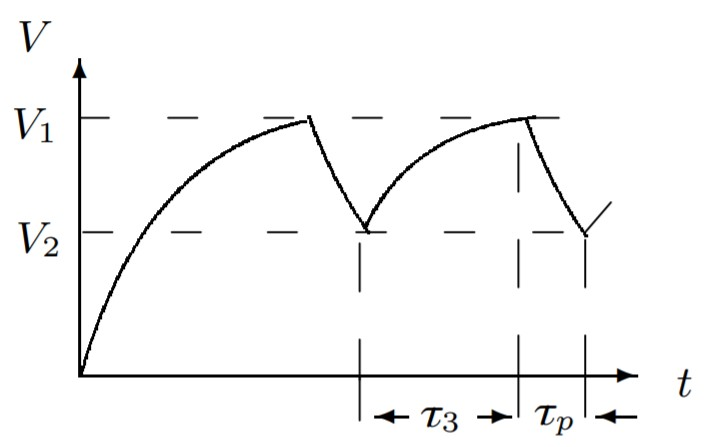
\includegraphics[width=5cm]{ris4.jpg}
	\caption{\textit{Осциллограмма релаксационных колебаний}}
	\label{ris4}
\end{wrapfigure}

Рассмотрим, как происходит колебательный процесс. Пусть в начале опыта ключ К разомкнут (рис. \ref{ris2}) и $ V = 0 $. Замкнём ключ. Конденсатор $ C $ начинает заряжаться через сопротивление $ R $, напряжение на нём увеличивается (рис. \ref{ris4}). Как только оно достигнет напряжения зажигания $ V_1 $, лампа начинает проводить ток, причём прохождение тока сопровождается разрядкой конденсатора. В самом деле, батарея $ U $, подключённая через большое сопротивление $ R $, не может поддерживать необходимую для горения лампы величину тока. Во время горения лампы конденсатор разряжается, и когда напряжение на нём достигнет потенциала гашения, лампа перестанет проводить ток, а конденсатор вновь начнёт заряжаться. Возникают релаксационные колебания с амплитудой, равной $ (V_1-V_2) $.

Рассчитаем период колебаний. Полное время одного периода колебаний $ T $ состоит из суммы времени зарядки $ \tau_\text{з} $ и времени разрядки $ \tau_\text{р} $, но если сопротивление $ R $ существенно превосходит сопротивление зажжённой лампы, то $ \tau_\text{з} \gg \tau_\text{р}  $ и $ T \approx \tau_\text{з} $ (этим случаем мы и ограничимся).

Во время зарядки конденсатора лампа не горит ($ I(V) = 0 $), и уравнение \eqref{1} приобретает вид

\begin{equation}\label{4}
RC\frac{dV}{dt}=U-V
\end{equation}

Будем отсчитывать время с момента гашения лампы, так что $ V = V_2 $ при $ t=0 $. (рис. \ref{ris4}). Решив уравнение \eqref{4}, найдём

\begin{equation}\label{5}
V = U - (U - V_2)e^{-t/RC}.
\end{equation}

В момент зажигания t = $ \tau_\text{з} $, $ V = V_1 $, поэтому

\begin{equation}\label{6}
V_1=U-(U-V_2)e^{-\tau_\text{з}/RC}.
\end{equation}

Из уравнений \eqref{5} и \eqref{6} нетрудно найти период колебаний:
\label{form}
\begin{equation}\label{7}
T\approx\tau_\text{з}=RC\ln\frac{U-V_2}{U-V_1}
\end{equation}

Данная теория справедлива лишь в тех случаях, когда в схеме установлена достаточно большая ёмкость и когда период колебаний существенно больше времени развития разряда и времени деионизации (практически $ \gg 10^{-5} $ с). Кроме того, потенциал гашения $ V_2 $, взятый из статической вольт-амперной характеристики, может отличаться от потенциала гашения лампы, работающей в динамическом режиме релаксационных колебаний.

\section{Ход работы}

\subsection{Исследование вольт-амперной характеристики стабилитрона}

Для того, чтобы предотвратить перегорание стабилитрона, последовательно лампочке припаян резистор номиналом $ r = 5,1 $ кОм. Измерим ВАХ данного элемента при помощи вольтметра, амперметра и источника питания. полученные результаты занесём в таблицу \ref{tab:tab1}.

\begin{table}[H]
	\centering
	\begin{tabular}{|c|c|c|c|c|c|c|c|}
		\hline
		$ U $, В     & $ I $, мА    & $ U $, В     & $ I $, мА     & $ U $, В     & $ I $, мА     & $ U $, В     & $ I $, мА     \\ \hline
		5,67  & 0,01 & 91,80  & 3,84  & 248,78 & 33,61 & 150,98 & 14,95 \\ \hline
		11,35 & 0,01 & 102,13 & 5,78  & 275,76 & 38,75 & 129,32 & 11,06 \\ \hline
		21,76 & 0,01 & 116,48 & 8,48  & 292,57 & 41,82 & 116,23 & 8,45  \\ \hline
		34,21 & 0,01 & 127,65 & 10,58 & 265,71 & 36,85 & 101,69 & 5,74  \\ \hline
		47,00 & 0,01 & 141,73 & 13,79 & 249,46 & 33,70 & 93,36  & 4,17  \\ \hline
		57,15 & 0,02 & 160,92 & 16,79 & 225,85 & 29,19 & 81,90  & 2,11  \\ \hline
		64,13 & 0,02 & 179,71 & 19,78 & 205,18 & 25,54 & 71,77  & 0,79  \\ \hline
		80,34 & 0,02 & 199,28 & 24,19 & 193,41 & 23,20 & 73,31  & 0,01  \\ \hline
		82,34 & 0,02 & 212,14 & 26,62 & 182,43 & 21,64 & 87,90  & 3,11  \\ \hline
		87,75 & 0,02 & 231,45 & 30,30 & 169,14 & 18,36 & 72,76  & 0,44  \\ \hline
	\end{tabular}
	\caption{Результаты измерения ВАХ}
	\label{tab:tab1}
\end{table}

Нанесём полученные данные ВАХ для сборки <<стабилитрон-резистор>> на график.

\begin{center}
	\begin{tikzpicture}
	\begin{axis}[
	title={Вольт-амперная характеристика сборки <<стабилитрон-резистор>>},
	xlabel={$ U $, В},
	ylabel={$ I $, мА},
	legend pos=north west,
	xmajorgrids=true,
	ymajorgrids=true,
	grid style=dashed,
	width = 520,
	height = 300,
	%xmin = 300,
	%xmax = 120,
	%ymin =40,
	%ymax =135,
	]
	\legend{ 
		ВАХ,
	};
	\addplot+ [blue, only marks, mark size = 4pt,
	error bars/.cd,
	x dir=both, x explicit,
	y dir=both, y explicit, 
	] table [x = T, y = sigma, x error = dT, y error = ds,] {
		T	sigma    dT    ds            
		5.67	0.012	0.05	0.01
		11.35	0.012	0.05	0.01
		21.76	0.013	0.05	0.01
		34.21	0.013	0.05	0.01
		47	0.014	0.05	0.01
		57.15	0.015	0.05	0.01
		64.13	0.016	0.05	0.01
		80.34	0.017	0.05	0.01
		82.34	0.018	0.05	0.01
		87.75	0.018	0.05	0.01
		91.8	3.835	0.05	0.01
		102.13	5.78	0.05	0.01
		116.48	8.48	0.05	0.01
		127.65	10.58	0.05	0.01
		141.73	13.79	0.05	0.01
		160.92	16.79	0.05	0.01
		179.71	19.78	0.05	0.01
		199.28	24.19	0.05	0.01
		212.14	26.62	0.05	0.01
		231.45	30.3	0.05	0.01
		248.78	33.61	0.05	0.01
		275.76	38.75	0.05	0.01
		292.57	41.82	0.05	0.01
		265.71	36.85	0.05	0.01
		249.46	33.7	0.05	0.01
		225.85	29.19	0.05	0.01
		205.18	25.54	0.05	0.01
		193.41	23.2	0.05	0.01
		182.43	21.64	0.05	0.01
		169.14	18.363	0.05	0.01
		150.98	14.95	0.05	0.01
		129.32	11.06	0.05	0.01
		116.23	8.45	0.05	0.01
		101.69	5.74	0.05	0.01
		93.36	4.17	0.05	0.01
		81.9	2.11	0.05	0.01
		71.77	0.793	0.05	0.01
		73.31	0.007	0.05	0.01
		87.9	3.114	0.05	0.01
		72.76	0.443	0.05	0.01
		
		
	};
	\end{axis}
	\end{tikzpicture}
\end{center}

Также ниже представлена чать графика вблизи напряжения зажигания.

\begin{center}
	\begin{tikzpicture}
	\begin{axis}[
	title={Вольт-амперная характеристика сборки <<стабилитрон-резистор>>},
	xlabel={$ U $, В},
	ylabel={$ I $, мА},
	legend pos=north west,
	xmajorgrids=true,
	ymajorgrids=true,
	grid style=dashed,
	width = 520,
	height = 400,
	%xmin = 300,
	xmax = 120,
	%ymin =40,
	%ymax =135,
	]
	\legend{ 
		ВАХ,
	};
	\addplot+ [blue, only marks, mark size = 4pt,
	error bars/.cd,
	x dir=both, x explicit,
	y dir=both, y explicit, 
	] table [x = T, y = sigma, x error = dT, y error = ds,] {
		T	sigma    dT    ds            
		5.67	0.012	0.05	0.01
		11.35	0.012	0.05	0.01
		21.76	0.013	0.05	0.01
		34.21	0.013	0.05	0.01
		47	0.014	0.05	0.01
		57.15	0.015	0.05	0.01
		64.13	0.016	0.05	0.01
		80.34	0.017	0.05	0.01
		82.34	0.018	0.05	0.01
		87.75	0.018	0.05	0.01
		91.8	3.835	0.05	0.01
		102.13	5.78	0.05	0.01
		116.48	8.48	0.05	0.01
		127.65	10.58	0.05	0.01
		141.73	13.79	0.05	0.01
		160.92	16.79	0.05	0.01
		179.71	19.78	0.05	0.01
		199.28	24.19	0.05	0.01
		212.14	26.62	0.05	0.01
		231.45	30.3	0.05	0.01
		248.78	33.61	0.05	0.01
		275.76	38.75	0.05	0.01
		292.57	41.82	0.05	0.01
		265.71	36.85	0.05	0.01
		249.46	33.7	0.05	0.01
		225.85	29.19	0.05	0.01
		205.18	25.54	0.05	0.01
		193.41	23.2	0.05	0.01
		182.43	21.64	0.05	0.01
		169.14	18.363	0.05	0.01
		150.98	14.95	0.05	0.01
		129.32	11.06	0.05	0.01
		116.23	8.45	0.05	0.01
		101.69	5.74	0.05	0.01
		93.36	4.17	0.05	0.01
		81.9	2.11	0.05	0.01
		71.77	0.793	0.05	0.01
		73.31	0.007	0.05	0.01
		87.9	3.114	0.05	0.01
		72.76	0.443	0.05	0.01
		
		
	};
	\end{axis}
	\end{tikzpicture}
\end{center}

Теперь получим ВАХ стабилитрона, вычитая для этого из показаний вольтметра падение напряжения на резисторе. Полученные результаты вычислений занесём в таблицу \ref{tab:tab2}.

\begin{table}[H]
	\centering
	\begin{tabular}{|c|c|c|c|c|c|c|c|}
		\hline
		$ U $, В     & $ I $, мА    & $ U $, В     & $ I $, мА     & $ U $, В     & $ I $, мА     & $ U $, В     & $ I $, мА     \\ \hline
		5,61  & 0,01 & 72,24 & 3,84  & 77,37 & 33,61 & 74,74 & 14,95 \\ \hline
		11,29 & 0,01 & 72,65 & 5,78  & 78,14 & 38,75 & 72,91 & 11,06 \\ \hline
		21,69 & 0,01 & 73,23 & 8,48  & 79,29 & 41,82 & 73,14 & 8,45  \\ \hline
		34,14 & 0,01 & 73,69 & 10,58 & 77,78 & 36,85 & 72,42 & 5,74  \\ \hline
		46,93 & 0,01 & 71,40 & 13,79 & 77,59 & 33,70 & 72,09 & 4,17  \\ \hline
		57,07 & 0,02 & 75,29 & 16,79 & 76,98 & 29,19 & 71,14 & 2,11  \\ \hline
		64,05 & 0,02 & 78,83 & 19,78 & 74,93 & 25,54 & 67,73 & 0,79  \\ \hline
		80,25 & 0,02 & 75,91 & 24,19 & 75,09 & 23,20 & 73,27 & 0,01  \\ \hline
		82,25 & 0,02 & 76,38 & 26,62 & 72,07 & 21,64 & 72,02 & 3,11  \\ \hline
		87,66 & 0,02 & 76,92 & 30,30 & 75,49 & 18,36 & 70,50 & 0,44  \\ \hline
	\end{tabular}
	\caption{Результаты измерения ВАХ стабилитрона}
	\label{tab:tab2}
\end{table}

Нанесём полученные данные на график.

\begin{center}
	\begin{tikzpicture}
	\begin{axis}[
	title={Вольт-амперная характеристика стабилитрона},
	xlabel={$ U $, В},
	ylabel={$ I $, мА},
	legend pos=north west,
	xmajorgrids=true,
	ymajorgrids=true,
	grid style=dashed,
	width = 520,
	height = 300,
	%xmin = 300,
	%xmax = 120,
	%ymin =40,
	%ymax =135,
	]
	\legend{ 
		ВАХ,
	};
	\addplot+ [blue, only marks, mark size = 4pt,
	error bars/.cd,
	x dir=both, x explicit,
	y dir=both, y explicit, 
	] table [x = T, y = sigma, x error = dT, y error = ds,] {
		T	sigma    dT    ds            
		5.6088	0.012	1	0.05
		11.2888	0.012	1	0.05
		21.6937	0.013	1	0.05
		34.1437	0.013	1	0.05
		46.9286	0.014	1	0.05
		57.0735	0.015	1	0.05
		64.0484	0.016	1	0.05
		80.2533	0.017	1	0.05
		82.2482	0.018	1	0.05
		87.6582	0.018	1	0.05
		72.2415	3.835	1	0.05
		72.652	5.78	1	0.05
		73.232	8.48	1	0.05
		73.692	10.58	1	0.05
		71.401	13.79	1	0.05
		75.291	16.79	1	0.05
		78.832	19.78	1	0.05
		75.911	24.19	1	0.05
		76.378	26.62	1	0.05
		76.92	30.3	1	0.05
		77.369	33.61	1	0.05
		78.135	38.75	1	0.05
		79.288	41.82	1	0.05
		77.775	36.85	1	0.05
		77.59	33.7	1	0.05
		76.981	29.19	1	0.05
		74.926	25.54	1	0.05
		75.09	23.2	1	0.05
		72.066	21.64	1	0.05
		75.4887	18.363	1	0.05
		74.735	14.95	1	0.05
		72.914	11.06	1	0.05
		73.135	8.45	1	0.05
		72.416	5.74	1	0.05
		72.093	4.17	1	0.05
		71.139	2.11	1	0.05
		67.7257	0.793	1	0.05
		73.2743	0.007	1	0.05
		72.0186	3.114	1	0.05
		70.5007	0.443	1	0.05
		
	};
	\end{axis}
	\end{tikzpicture}
\end{center}

При помощи полученной характеристики можем определить потенциалы зажигания и гашения и соответствующие им токи. Таким образом, получаем

\[ V_1 = (79,29 \pm 0,05) \text{ В}, \qquad I_1 = (41,82 \pm 0,01) \text{ мА}, \]
\[ V_2 = (72,76 \pm 0,05) \text{ В}, \qquad I_2 = (0,44 \pm 0,01) \text{ мА}. \]

\label{nums}

Полученные данные понадобятся нам в следующей части работы.

\subsection{Осциллограммы релаксационных колебаний}

Собрав схему, согласно рис. \ref{ris2}, оценим отношение между временем зарядки $ \tau_\text{з} $ и  временем разрядки $ \tau_\text{р} $ при помощи осциллографа. Получим на экране осциллографа картину колебаний.

\begin{figure}[H]
	\begin{center}
		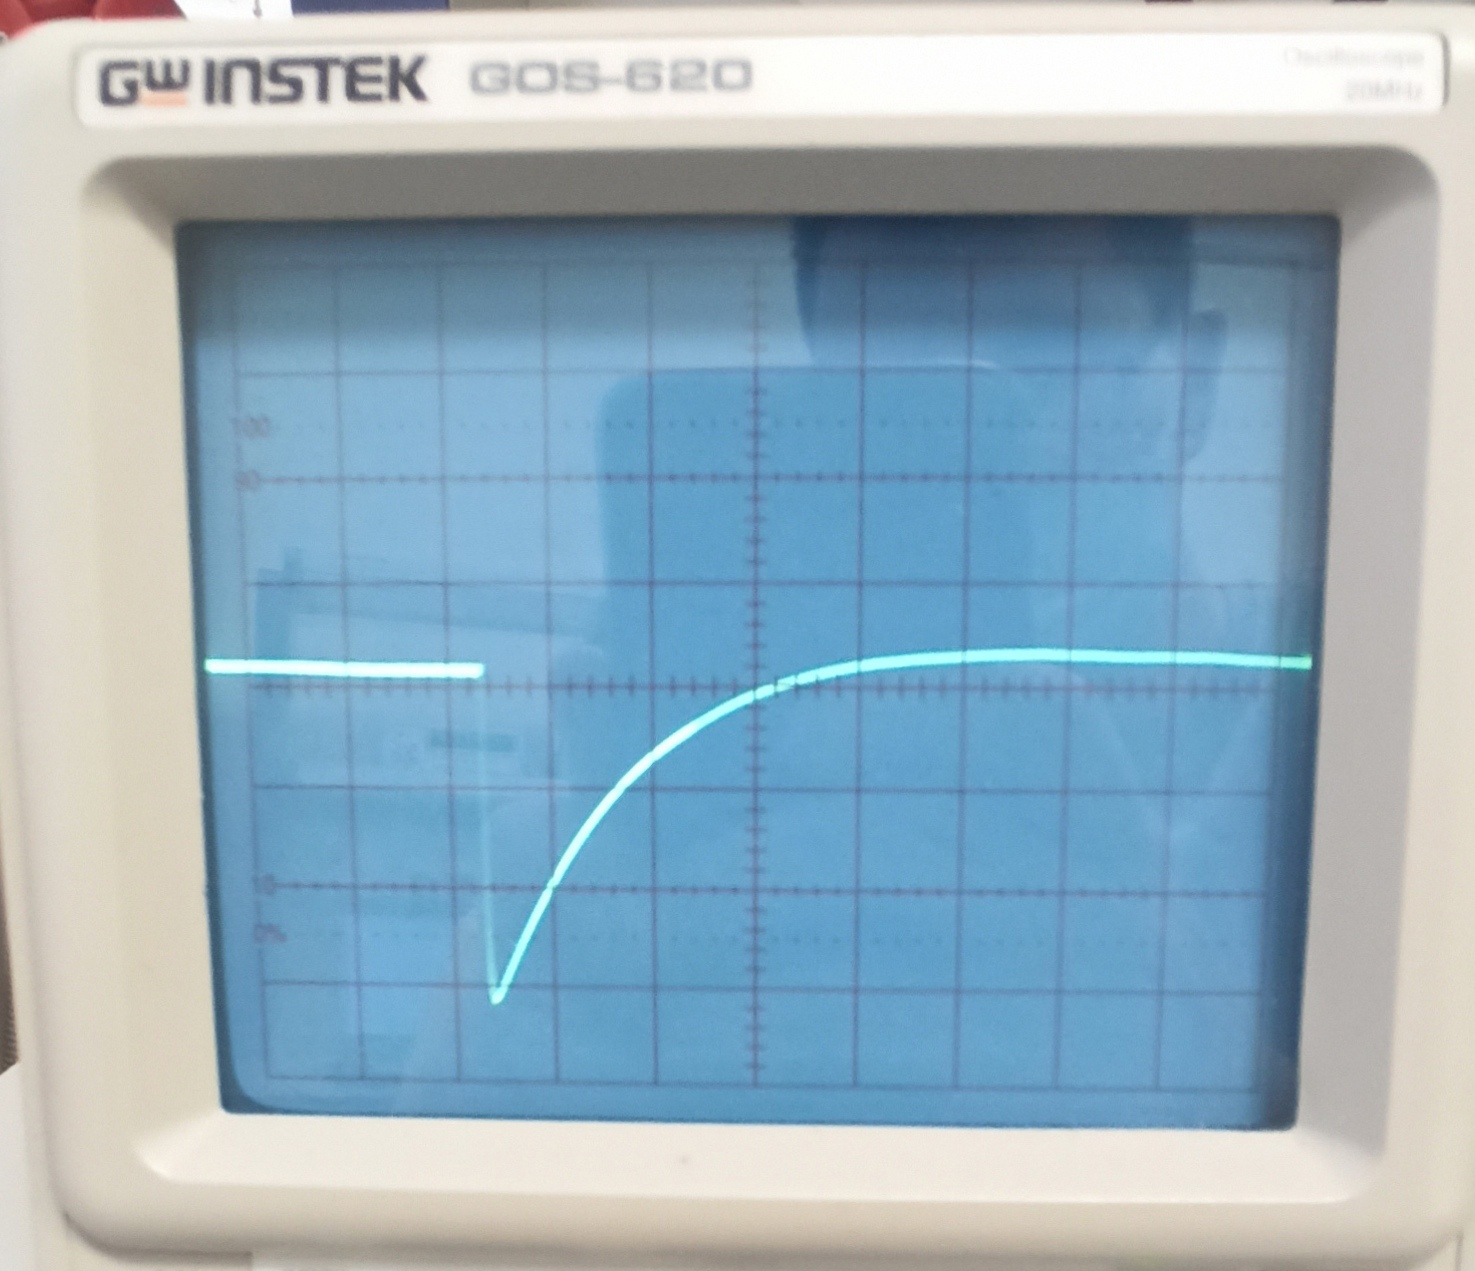
\includegraphics[width=8cm]{ris5.jpg}
	\end{center}
	\caption{\textit{Картина колебаний}}
	\label{ris5}
\end{figure}

При помощи осциллографа определяем $ \tau_\text{р} \approx 1$ мс и $ \tau_\text{р} \approx 60 $ мс. Таким образом, в контексте нашей работы можно считать, что $ \tau_\text{р} \ll \tau_\text{р} $ и $ T \approx \tau_\text{з} $, что делает возможным использование приведённой выше теории и, в частности, формулы \eqref{7}.

Уменьшая сопротивление, определим $ R_\text{кр} $, при котором пропадают колебания. Колебания затухают при $ R_\text{кр}^\text{эксп} \approx 100 $ кОм. При этом теоретическое значение критического напряжения, расчитанное по \eqref{3} для текущего напряжения $ U = 105,78 $ В равно $ R_\text{кр}^\text{теор} = 74,5 \pm 0,5 $ кОм. Расходимость результатов может быть объяснена наличием дополнительного резистора, подключенного последовательно с стабилитроном, что и делает данные теоретические вычисления неточными. Однако, полученный ответ совпадает по порядку величины с практическими данными.

Также колебания пропадают и при увеличении $ U $ при постоянном $ R $. Так, колебания затухают при $ U = 113,3 $ В и $ R = 120 $ кОм.

\subsection{Определение частоты колебаний при помощи фигур Лиссажу}

\subsubsection{Получение фигур Лиссажу}

Сначала проверим возможность получения фигур Лиссажу на экране осциллографа. Установим $ C = 5\cdot10^{-2} $ мкФ и $ R = 900 $ кОм. Изменяя частоту звукового генератора, получим на экране изображения фигур Лиссажу. Они представлены ниже.

\begin{table}[H]
	\centering
	\begin{tabular}{|c|c|c|}
		\hline
	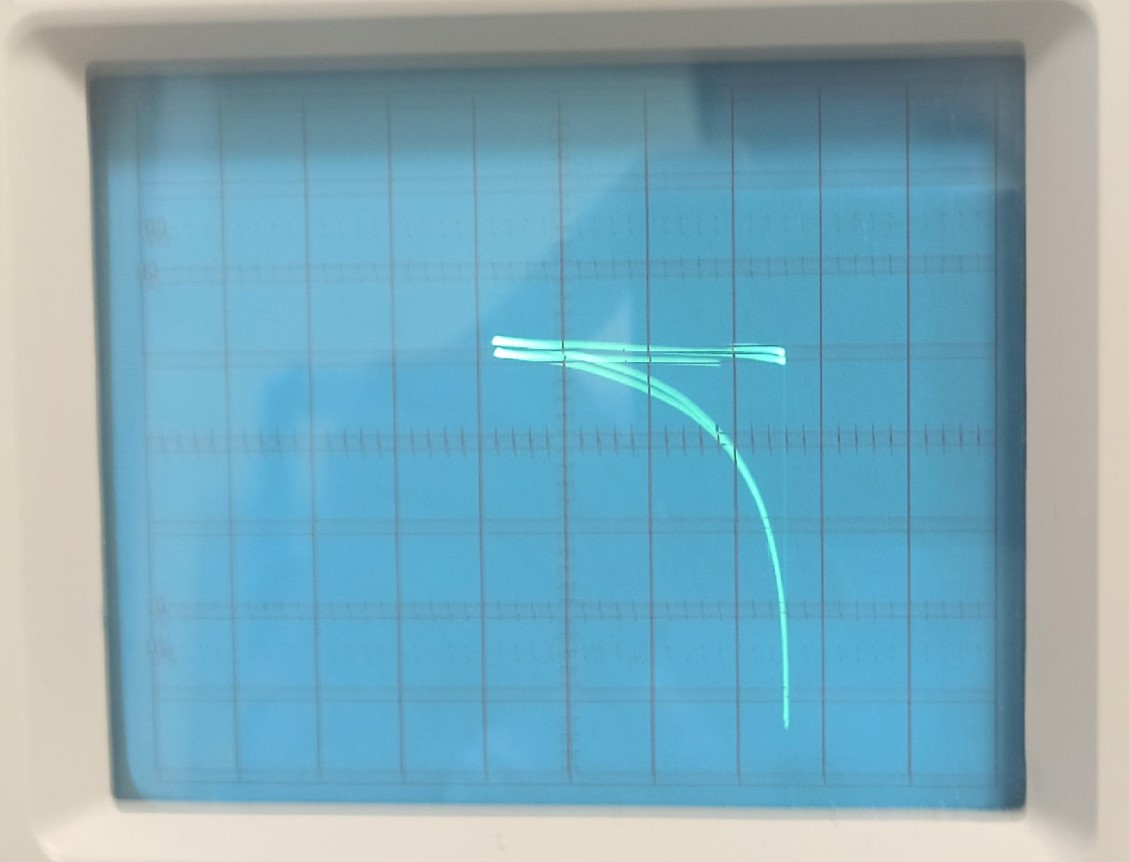
\includegraphics[width=0.33\textwidth]{ris6.jpg}	& 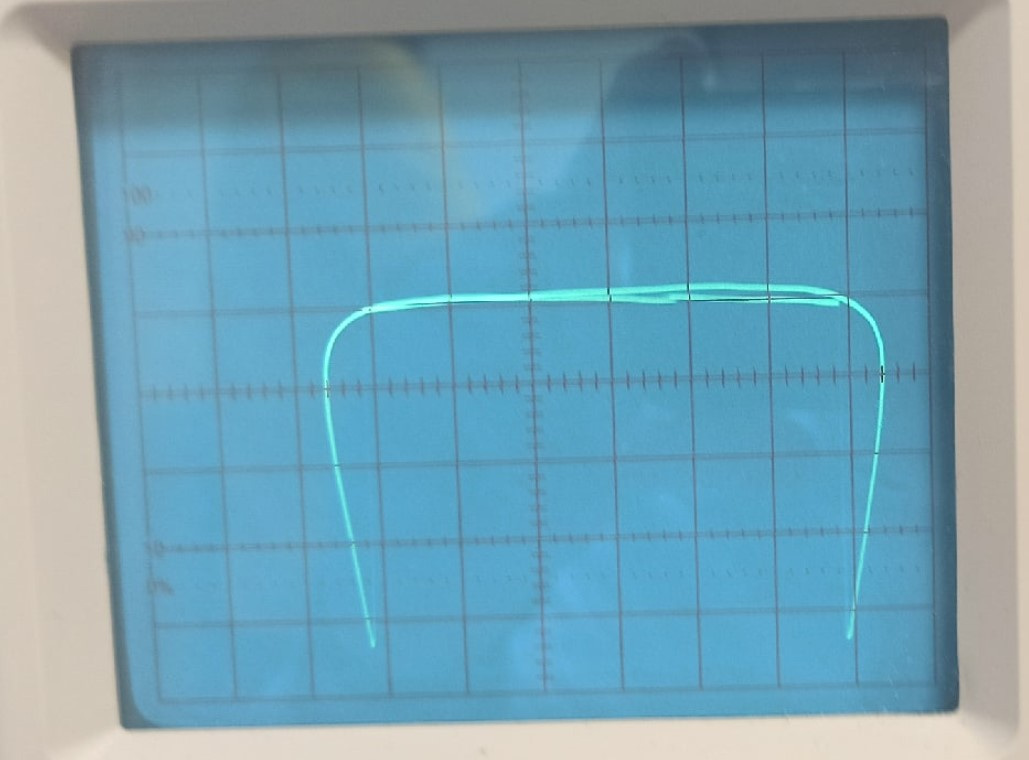
\includegraphics[width=0.33\textwidth]{ris7.jpg} & 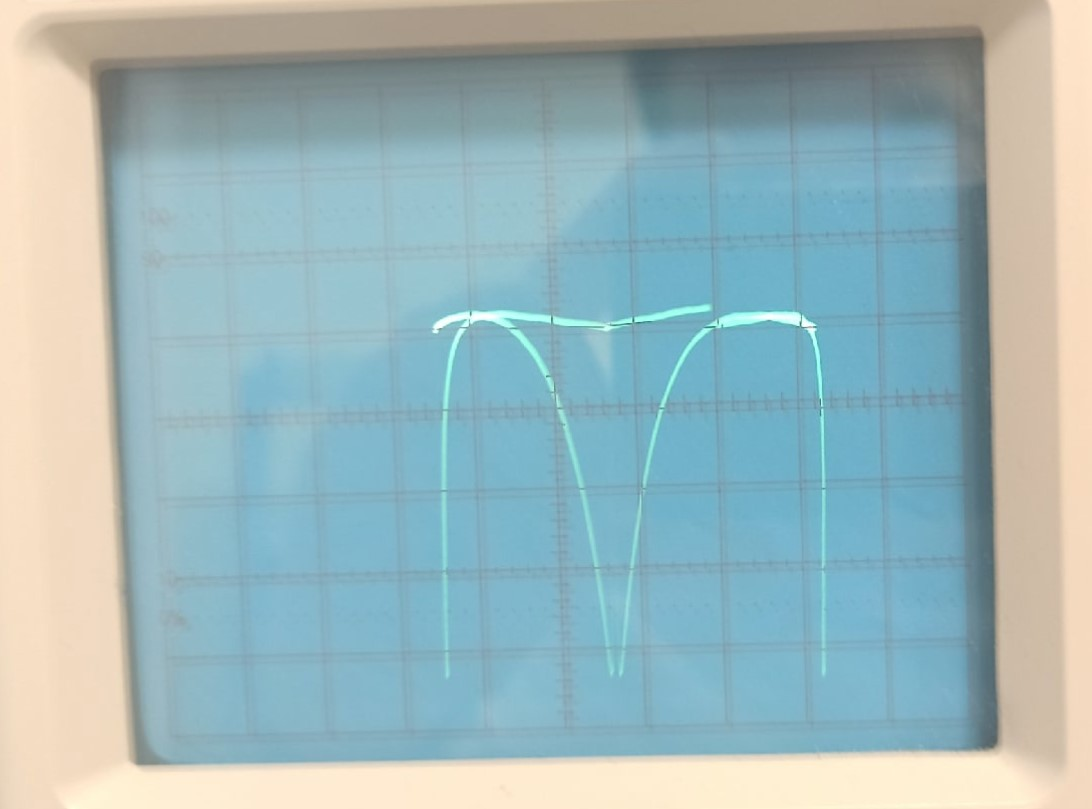
\includegraphics[width=0.33\textwidth]{ris8.jpg} \\ \hline
	1:1	& 1:2 & 1:3 \\ \hline
	\end{tabular}
\end{table}

\subsubsection{Изучение зависимости периода колебаний от ёмкости}

В данном разделе все измерения будем проводить при напряжении источника $ U = 105,48 $ В.

Для дальнейших расчётов вычислим постоянный коэффициент $ a = \ln((U - V_2)/(U-V_1)) $. Для этого воспользуемся $ V_1 $ и $ V_2 $, вычисленные в разделе \ref{nums}.

Погрешность вычисления данного коэффициента рассчитаем по следующей формуле:

\[ \sigma_a = \sqrt{\left(\frac{\partial a}{\partial U}\sigma_U\right)^2+\left(\frac{\partial a}{\partial V_1}\sigma_{V_1}\right)^2+\left(\frac{\partial a}{\partial V_2}\sigma_{V_2}\right)^2} \]

В итоге получаем:

\[ \boxed{a = 0,22 \pm 0,04} \]

Теперь при помощи фигур Лиссажу снимем зависимость частоты колебаний от ёмкости конденсатора. Полученные результаты занесём в таблицу \ref{tab:tab3}.

\begin{table}[H]
	\centering
	\begin{tabular}{|c|c|c|c|c|c|c|}
		\hline
		$ C $, нФ & 50  & 40  & 35  & 30   & 20   & 10   \\ \hline
		$ f $, Гц & 567 & 779 & 829 & 1087 & 1810 & 4670 \\ \hline
	\end{tabular}
	\caption{Результаты измерений}
	\label{tab:tab3}
\end{table}

По полученным данным построим график зависимости периода колебаний $ T $ от ёмкости $ C $. Для удобства немного преобразуем числа, занесём их в таблицу \ref{tab:tab4}.

\begin{table}[H]
	\centering
	\begin{tabular}{|c|c|c|c|c|c|c|}
		\hline
		$ C $, нФ    & 50   & 40   & 35   & 30   & 20   & 10   \\ \hline
		$ T $, мс    & 1,76 & 1,28 & 1,21 & 0,92 & 0,55 & 0,21 \\ \hline
		$ \sigma_T $, мс & 0,08 & 0,04 & 0,04 & 0,02 & 0,01 & 0,01 \\ \hline
	\end{tabular}
	\caption{Данные для построения графика}
	\label{tab:tab4}
\end{table}

По полученным данным построим график зависимости периода колебаний и аппроксимируем его уравнением вида $ y = kx+b $.


\begin{center}
	\begin{tikzpicture}
	\begin{axis}[
	title={Зависимость периода колебаний $ T $ от ёмкости $ C $},
	xlabel={$ C $, нФ},
	ylabel={$ T $, мс},
	legend pos=north west,
	xmajorgrids=true,
	ymajorgrids=true,
	grid style=dashed,
	width = 520,
	height = 300,
	xmin = 0,
	%xmax = 120,
	%ymin =40,
	%ymax =135,
	]
	\legend{ 
		,Экспериментальная зависимость,
		Теоретическая зависимость,
	};
	\addplot+ [blue, only marks, mark size = 4pt,
	error bars/.cd,
	x dir=both, x explicit,
	y dir=both, y explicit, 
	] table [x = T, y = sigma, x error = dT,] {
		T	sigma    dT          
		50	1.76366843	0.077763158
		40	1.283697047	0.041196953
		35	1.206272618	0.036377341
		30	0.919963201	0.021158307
		20	0.552486188	0.007631025
		10	0.214132762	0.001146321
	};
	\addplot [red, domain=9:52, line width =3.2pt] {0.03548 * x - 0.14093};
	\addplot [black, domain=9:52, line width =3.2pt] {0.041300139 * x};
	
	\end{axis}
	\end{tikzpicture}
\end{center}

В результате аппроксимации получаем

\[ \boxed{k_\text{эксп} = (35 \pm 1) \text{ кОм}} \]

Исходя из теоретических данных по формуле \eqref{7} получаем

\[ \boxed{k_\text{теор} = (41 \pm 10) \text{ кОм}} \]

\subsubsection{Изучение зависимости периода колебаний от сопротивления}

Аналогичные вычисления проведём при постоянной ёмкости и изменяющем сопротивлении. В ходе эксперимента оставим постоянной ёмкость $ C = 50 $ нФ. При помощи фигур Лиссажу снимем зависимость частоты колебаний от сопротивления. Полученные данные занесём в таблицу \ref{tab:tab5}.

\begin{table}[H]
	\centering
	\begin{tabular}{|c|c|c|c|c|c|c|c|c|c|c|c|c|c|c|c|c|}
		\hline
		$ R $, кОм     & 900  & 800  & 700 & 600 & 500 & 400 & 300 & 200 & 250 & 350 & 450 & 550 & 650 & 750 & 850  & 150 \\ \hline
		$ T $, мс     & 13,2 & 10,6 & 8,3 & 6,5 & 4,7 & 3,4 & 2,3 & 1,4 & 1,8 & 2,7 & 3,8 & 5,1 & 6,5 & 8,5 & 10,9 & 1,0 \\ \hline
		$ \sigma_T $, мс & 1,3  & 1,1  & 0,8 & 0,6 & 0,5 & 0,3 & 0,2 & 0,1 & 0,2 & 0,3 & 0,4 & 0,5 & 0,6 & 0,8 & 1,1  & 0,1 \\ \hline
	\end{tabular}
	\caption{Результаты измерений}
	\label{tab:tab5}
\end{table}

По полученным данным построим график зависимости периода колебаний $ T $ от сопротивления $ R $. Аппроксимируем зависимость уравнением вида $ y = kx + b $.


\begin{center}
	\begin{tikzpicture}
	\begin{axis}[
	title={Зависимость периода колебаний $ T $ от сопротивления $ R $},
	xlabel={$ R $, кОм},
	ylabel={$ T $, мс},
	legend pos=north west,
	xmajorgrids=true,
	ymajorgrids=true,
	grid style=dashed,
	width = 520,
	height = 300,
	xmin = 0,
	%xmax = 120,
	%ymin =40,
	%ymax =135,
	]
	\legend{ 
		,Экспериментальная зависимость,
		Теоретическая зависимость,
	};
	\addplot+ [blue, only marks, mark size = 4pt,
	error bars/.cd,
	x dir=both, x explicit,
	y dir=both, y explicit, 
	] table [x = T, y = sigma, x error = dT,] {
		T	sigma    dT          
		900	13.2	1.3
		800	10.6	1.1
		700	8.3	0.8
		600	6.5	0.6
		500	4.7	0.5
		400	3.4	0.3
		300	2.3	0.2
		200	1.4	0.1
		250	1.8	0.2
		350	2.7	0.3
		450	3.8	0.4
		550	5.1	0.5
		650	6.5	0.6
		750	8.5	0.8
		850	10.9	1.1
		150	1.0	0.1
		
	};
	\addplot [red, domain=100:920, line width =3.2pt] {0.01173 * x - 0.96904};
	\addplot [black, domain=100:920, line width =3.2pt] {0.011126625 * x};
	
	\end{axis}
	\end{tikzpicture}
\end{center}

После аппроксимации получаем 

\[ \boxed{k_\text{эксп} = (11,7 \pm 0,7)  \text{ нФ}} \]

Исходя из теоретических данных по формуле \eqref{7} получаем

\[ \boxed{k_\text{теор} = (11,2 \pm 2,9) \text{ нФ}} \]

\section{Обсуждение результатов и выводы}

В ходе выполнения работы были получены следующие результаты:

\begin{itemize}
	\item Была измерена вольт-амперная характеристика сборки стабилитрона и резистора. Затем была получена ВАХ для чистого стабилитрона. По полученным данным были рассчитаны напряжения загорания и тушения. Также полученные ВАХи были нанесены на графики. Полученные картины совпадают с теоретическими и дают адекватное представление о характере поведения элемента в цепи.
	\item При помощи осциллографа были изучены релаксационные колебания. По полученные картинам сигнала было произведено сравнение времени зарядки и разрядки $ \tau_\text{з}, \tau\text{р} $. Было установлено, что $ \tau_\text{з} \gg \tau_\text{р} $, что сделало возможным использование полученных в \ref{form} теоретических выкладок.
	\item Также было выяснено экспериментально значение $ R_\text{кр} $, при котором прекращаются колебания. Полученное практически значение не совпало с теоретическим, что могло произойти из-за наличия предохранительного резистора, который не учитывался при наших теоретических расчётах. Кроме того, в согласие с теорией, колебания затухали и при увеличении $ U $ при постоянном $ R $.
	\item При помощи осциллографа были получены фигуры Лиссажу колебаний, что сделало возможным определение их частоты. При помощ этого метода была исследована зависимость периода релаксационных колебаний от сопротивления $ R $ и ёмкости $ C $. Угловые коэффициенты наклона аппроксимированных зависимостей в пределах погрешностей совпадают с данными, полученными в ходе теоретических расчётов. При этом вертикальный сдвиг экспериментальной зависимости относительно теоретической может говорить о влиянии предохранительного резистора.
	\item Кроме того, при исследовании зависимости периода колебаний от сопротивления $ R $ на участке $ R > 700 $ кОм была обнаружено отклонение от теоретической линейной зависимости неизвестного генеза. Это может говорить о выходе за рамки приближений, которые были допущены при выведении теоретических зависимостей. Для получения полных результатов эта область нуждается в более тщательном исследовании.
\end{itemize}

Основной вклад в ошибку в этой работе внесла невозможность точной подстройки частоты звукового генератора для получения на экране осциллографа неподвижной и чёткой картины фигуры Лиссажу. Возможно, целесообразно заменить имеющийся аналоговый генератор на современный цифровой прибор с тем, чтобы значительно повысить точность эксперимента.








\end{document}